\section{Cây Merkle}
\subsection{Khái niệm cây Merkle}

Merkle Tree là một cấu trúc dữ liệu cây nhị phân được sử dụng trong một số loại hệ thống phân 
tán để đảm bảo tính toàn vẹn dữ liệu. 

Cấu trúc Merkle Tree là một cấu trúc dữ liệu cây nhị phân, trong đó mỗi nút lá của cây biểu diễn
một khối dữ liệu và mỗi nút cha của hai nút lá biểu diễn giá trị băm của hai khối dữ 
liệu liên tiếp. Các giá trị băm này được tính toán bằng cách sử dụng một thuật toán băm như 
SHA-256 hoặc SHA-3.


\begin{figure}[h]
    \centering
    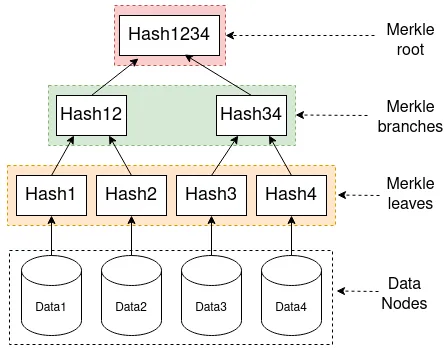
\includegraphics[width=0.6\textwidth]{images/Merkle_Tree.png}
    \caption{Merkle Tree }
    \label{fig:merkle_tree}
\end{figure}

Các giá trị băm của các cặp khối dữ liệu liên tiếp được sử dụng để tính toán giá trị băm của 
các nút cha tiếp theo. Quá trình này được lặp lại cho đến khi chỉ còn lại một giá trị băm duy 
nhất, được gọi là "root hash". Các giá trị băm này được sử dụng để đảm bảo tính toàn vẹn của 
dữ liệu được lưu trữ trong cây.

Số nút lá của cây Merkle là luỹ thừa của 2 (2,4,8,16,32,...). Nếu số nút lá của cây không
đủ, thì sẽ sử dụng dữ liệu cuối cùng để đại diện cho khối dữ liệu còn thiếu.



Một cây Merkle có thể được sử dụng để giảm thiểu khối lượng dữ liệu cần truyền qua mạng khi 
xác minh tính toàn vẹn của một tập hợp lớn các khối dữ liệu. Thay vì truyền toàn bộ dữ liệu qua
mạng, chỉ cần truyền giá trị băm của các khối dữ liệu và giá trị băm của các nút cha để xác minh tính toàn vẹn của dữ liệu.

Một trong những ứng dụng phổ biến nhất của cây Merkle là trong blockchain. Trong blockchain,
các giao dịch được kết hợp với nhau để tạo thành một khối, và các khối này được kết hợp với nhau 
để tạo thành một cây Merkle. Các thợ đào sẽ sử dụng giá trị băm của cây Merkle để xác minh tính 
toàn vẹn của khối, giúp ngăn chặn các giao dịch giả mạo hoặc thay đổi dữ liệu trên blockchain.


\subsection{Merkle Root}

Merkle Root là giá trị băm  của nút gốc trong cây Merkle. Nó được tính toán 
bằng cách kết hợp giá trị băm của các nút cha trong cây Merkle.

Trong blockchain, Merkle Root được sử dụng để đại diện cho tất cả các giao dịch trong một khối. 
Các giao dịch được kết hợp với nhau để tạo thành một cây Merkle, và Merkle Root của cây này 
được sử dụng để đại diện cho toàn bộ khối trong blockchain.

Việc sử dụng Merkle Root giúp tăng tính toàn vẹn và bảo mật của blockchain. Nếu một giao dịch trong khối bị thay đổi, thì giá trị băm của Merkle Root sẽ thay đổi và blockchain sẽ không chấp nhận khối này. Do đó, Merkle Root giúp ngăn chặn các cuộc tấn công như giao dịch giả mạo hoặc thay đổi dữ liệu trên blockchain.

\subsection{Xác minh trong cây Merkle }

Chúng ta xác minh các giao dịch trên cây Merkle như thế nào?

Giả sử chúng ta có một cây Merkle với 8 nút lá thể hiện các giao dịch từ A đến H. Chúng ta sẽ sử dụng giá trị băm 
của các nút lá để xác minh tính toàn vẹn của dữ liệu. Giá trị băm của các nút lá 
được sử dụng để tính toán giá trị băm của các nút cha, và quá trình này được lặp 
lại cho đến khi chỉ còn lại một giá trị băm duy nhất, được gọi là ``root hash". 

\begin{figure}[h]
    \centering
    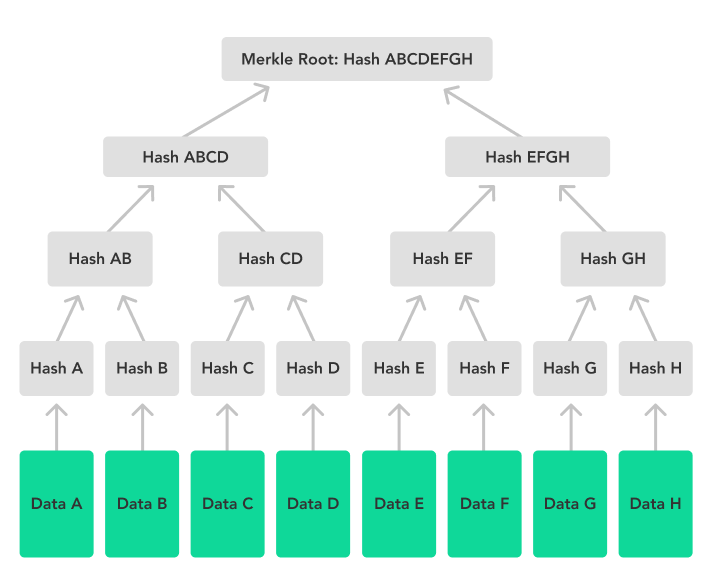
\includegraphics[width=0.6\textwidth]{images/merkle-tree-8levels.png}
    \caption{Cây Merkle 8 lá}
    \label{fig:merkle_tree_8levels}
\end{figure}


Giả sử ta cần xác minh một giao dịch, đầu tiên ta băm giao dịch và tìm kiếm kết quả
trong cây Merkle, nếu không tìm thấy kết quả thì thông tin giao dịch là giả. Nếu tìm được
một hàm băm lá trùng khớp với hàm băm ta vừa tính toán, thì thực hiện tính toán Merkle Root. 

Giả sử hàm băm thông tin giao dịch cần xác minh trùng khớp với Hash D.
Ta lấy thông tin Hash C để tính được Hash CD, sau đó lấy thông tin Hash AB để tính được Hash ABCD.
Cuối cùng sử dụng thông tin Hash EFGH kết hợp với Hash ABCD để tính được Merkle Root.

Cuối cùng so sánh Merkle Root vừa tính với giá trị Merkle Root được lưu trữ trong 
cây Merkle. Nếu hai giá trị này giống nhau, thì giao dịch là đúng, nếu không thì thông tin
giao dịch là giả.

